\documentclass[]{BasiliskReportMemo}
\usepackage{AVS}


\newcommand{\submiterInstitute}{Autonomous Vehicle Simulation (AVS) Laboratory,\\ University of Colorado}

\newcommand{\ModuleName}{thrMomentumDumping}
\newcommand{\subject}{Thrusting Firing Module to Cycle Through the RW Momentum Dumping}
\newcommand{\status}{initial document draft}
\newcommand{\preparer}{H. Schaub}
\newcommand{\summary}{This module reads in the desired impulse that each thruster must produce to create inertial momentum change to despin the RWs.   The output of the module is a setup of thruster firing times.  Each thruster can only fire for a maximum time that matches a single control period.  After this the thrusters are off for an integer number of control periods to let the RW re-stabilize the attitude about an inertial pointing scenario.    }


\begin{document}


\makeCover


%
%	enter the revision documentation here
%	to add more lines, copy the table entry and the \hline, and paste after the current entry.
%
\pagestyle{empty}
{\renewcommand{\arraystretch}{1.1}
\noindent
\begin{longtable}{|p{0.5in}|p{4.5in}|p{1.14in}|}
\hline
{\bfseries Rev}: & {\bfseries Change Description} & {\bfseries By} \\
\hline
Draft & Initial document creation & H. Schaub \\
1.0 & Document update after code review & H. Schaub \\
\hline

\end{longtable}
}

\newpage
\setcounter{page}{1}
\pagestyle{fancy}

\tableofcontents
~\\ \hrule ~\\

\begin{figure}[htb]
	\centerline{
	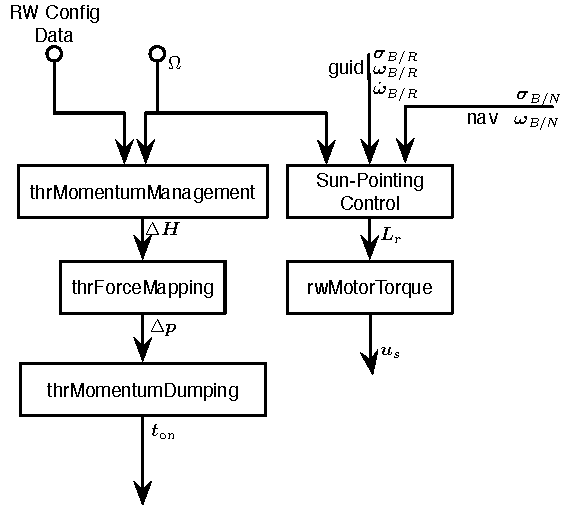
\includegraphics[]{Figures/rwMomentumOverview}
	}
	\caption{Overview of the Modules Used to Perform Reaction Wheel Angular Momentum Dumping.}
	\label{fig:Fig1}
\end{figure}

\section{Module Description}
\subsection{Overall RW Momentum Management Outline}
To manage the Reaction Wheel (RW) angular momentum build-up over time, a thruster-based momentum dumping strategy is used. Assume the spacecraft contains $N_{\text{RW}}$ RWs, and $M_{\text{thr}}$ thrusters.  Figure~\ref{fig:Fig1} illustrates how the momentum dumping will occur simultaneously with an inertial pointing control solution.   The output of {\tt thrMomentumManagement} module is a $\Delta \bm H$ vector.  This output is then mapped into a thruster impulse request using the {\tt thrForceMapping} module.  Note that this latter module is designed to map a control torque vector into thruster forces.  If the input torque and output force sets are multiplied by time,  the same module also functions to map a desired angular momentum changes vector $\Delta H$ into a set of thruster impulse requests.  The final module {\tt thrMomentumDumping} in the series takes the thruster impulse requests and determines a thruster firing sequence to achieve this desired momentum change.  The spacecraft attitude is held constant by simultaneously having a RW control module holding an inertial attitude.  The process of holding the desired attitude leads to the RWs despinning to the desired level due the external thruster disturbances.  




\begin{figure}[!t]
	\centerline{
	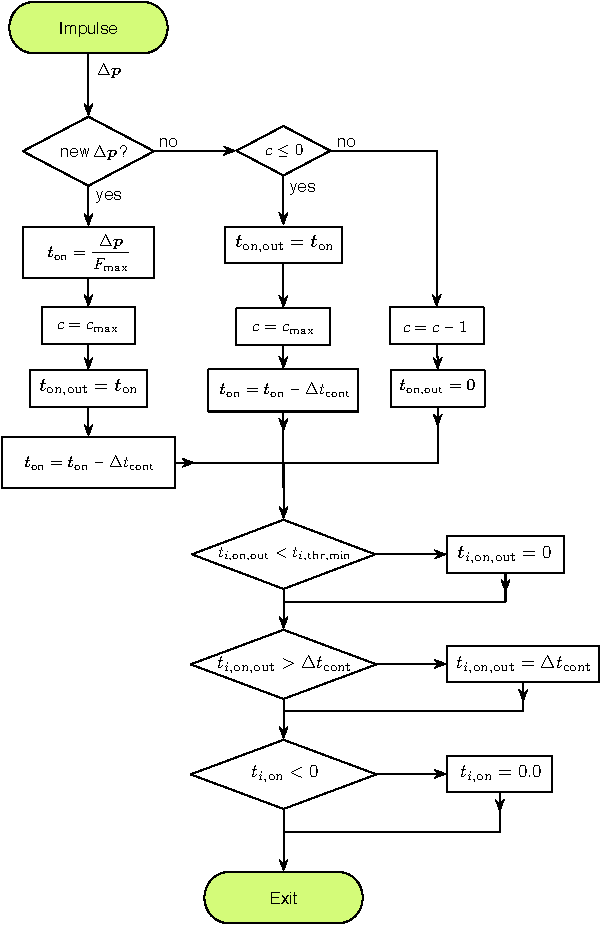
\includegraphics[]{Figures/rwMomentumDumping}
	}
	\caption{Overview of the Reaction Wheel Angular Momentum Dumping Module Logic.}
	\label{fig:Fig2}
\end{figure}


\subsection{Momentum Management Algorithm}
The following module algorithm logic is presented as a flow-diagram in Figure~\ref{fig:Fig2}.  This modules receives the vector of thruster impulses $\Delta\bm p$ from a thruster mapping module.  It first checks to see if this $\Delta\bm p$ is new by comparing the time tag of the input message with the time tag of the last used thruster impulse message.  If yes,  the overall thruster on-time values are computed using
\begin{equation}
	\bm t_{i,\text{on}} = \frac{\Delta \bm p}{F_{i,\text{max}}}
\end{equation}
where $F_{i,\text{max}}$ is the maximum thrust force achievable with the on-off type thruster.  These on-times are copied to the output thruster on-times, and the thruster cycling counter is reset.  

If the $\Delta\bm p$ message is not new, then the counter flag is checked.  If the counter is strictly positive, the thrusters should be off to allow for the RW to stabilize the orientation.  In this case the output thruster times are set to zero, and the counter is decremented, and the remaining required thruster on-times are decremented by the control time period.

If the counter flag reaches zero it is time to fire the required thrusters again to implement the next chunk of the required thruster impulse.  The output thrust on times are set to the remaining thruster on times, the counter is reset, and the remaining thruster on times is decremented again by the control period.

Finally, the thruster on times are checked to be greater than the thruster minimum firing time, or the output time is set to zero.  Similarly, if the required thruster on time is larger than a control period, the thruster on time is set equal to the control period.  This ensures that the thrusters will fire for a single control period duration only before returning to an off-mode.  The final check is to see if the thruster on-time remainders are negative, in which case they are reset to zero.



\begin{figure}[h]
	\centerline{
		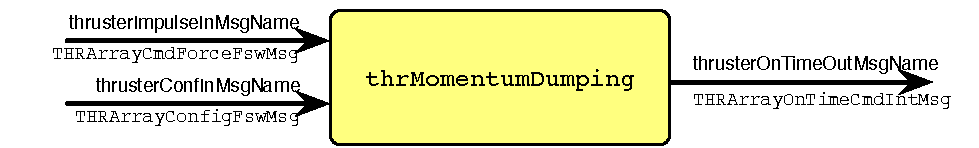
\includegraphics{Figures/moduleImg}
	}
	\caption{Illustration of the module input and output messages.}
	\label{fig:moduleImg}
\end{figure}





\subsection{Module Messages}
The module input and output messages are illustrated in Figure~\ref{fig:moduleImg}.  The module has a single output message of type {\tt THRArrayOnTimeCmdIntMsg} which contains the desired thruster burn times for the next control cycle.

There are 2 required input messages.  The message of type {\tt THRArrayConfigFswMsg} is read in during the {\tt Reset()} method and provides the thruster configuration states.  The message of type {\tt THRArrayCmdForceFswMsg} provides the currently requested thruster impulse values and is read in during the {\tt Update()} method.

\subsection{{\tt Reset()} Method}
The {\tt Reset()} method reads in the thruster message, and then resets dumping counter flag.  The stored thruster on time remainders and the request thruster impulse arrays are reset to zero.  Further, the thruster impulse request input message is red to see if an old message exists.  If yes, then the module variable tracking the time tag of the last impulse request is reset to this current message time tag. This avoids an old message being used after a reset.  If the input message has never been written, then the prior message time tag is set to zero.









\section{Module Functions}
\begin{itemize}
	\item \textbf{Keep checking for new thruster impulse requests}: If a new thruster impulse message is read in, then the momentum dumping cycle resumes again.
	\item \textbf{Create an output message with the desired thruster on-times}: The output is used to control the thruster burn duration.
\end{itemize}

\section{Module Assumptions and Limitations}
The module assumes the spacecraft is holding a steady inertial orientation during the momentum dumping maneuver.  










\section{Test Description and Success Criteria}
A module unit test is created which creates the required input messages and runs the module for a single iteration.  Two cases are considered where the minimum RWA momentum threshold is exceed or not.




\section{Test Parameters}
The simulation is setup with 8 thrusters  with identical $F_{\text{max}}$ values.  
The unit test verifies that the module output  message vector matches expected values.
\begin{table}[htbp]
	\caption{Error tolerance for each test.}
	\label{tab:errortol}
	\centering \fontsize{10}{10}\selectfont
	\begin{tabular}{ c | c } % Column formatting, 
		\hline\hline
		\textbf{Output Value Tested}  & \textbf{Tolerated Error}  \\ 
		\hline
		{\tt OnTimeRequest}        & 1e-05	   \\ 
		\hline\hline
	\end{tabular}
\end{table}




\section{Test Results}
All permutations of the test passed:
\begin{table}[h]
	\caption{Test results}
	\label{tab:results}
	\centering \fontsize{10}{10}\selectfont
	\begin{tabular}{c | c | c  } % Column formatting, 
		\hline\hline
		\textbf{resetCheck} & \textbf{largeMinFireTime}	&\textbf{Pass/Fail} \\ 
		\hline
	   False & 	  False 			& \input{AutoTeX/passFailFalseFalse} \\ 
	   False & True	   			& \input{AutoTeX/passFailFalseTrue} \\ 
	   True & False 	   			& \input{AutoTeX/passFailTrueFalse} \\ 
	   \hline\hline
	\end{tabular}
\end{table}









\section{User Guide}
The module configurable parameters include:
\begin{itemize}
	\item {{\tt maxCounterValue} Parameter}: 
This parameter dictates the number of control periods where the thrusters cycle off to allow the RWs to re-stabilize the orientation.  It must be set to a strictly positive value.  

	\item {{\tt thrMinFireTime} Parameter}: 
This parameter determines what the minimum thruster firing time is, provided in units of seconds.  
\end{itemize}



\end{document}
